\label{sec:results}

\subsection{Training Results}

%TC:ignore
\begin{figure}[h]
  \centering
  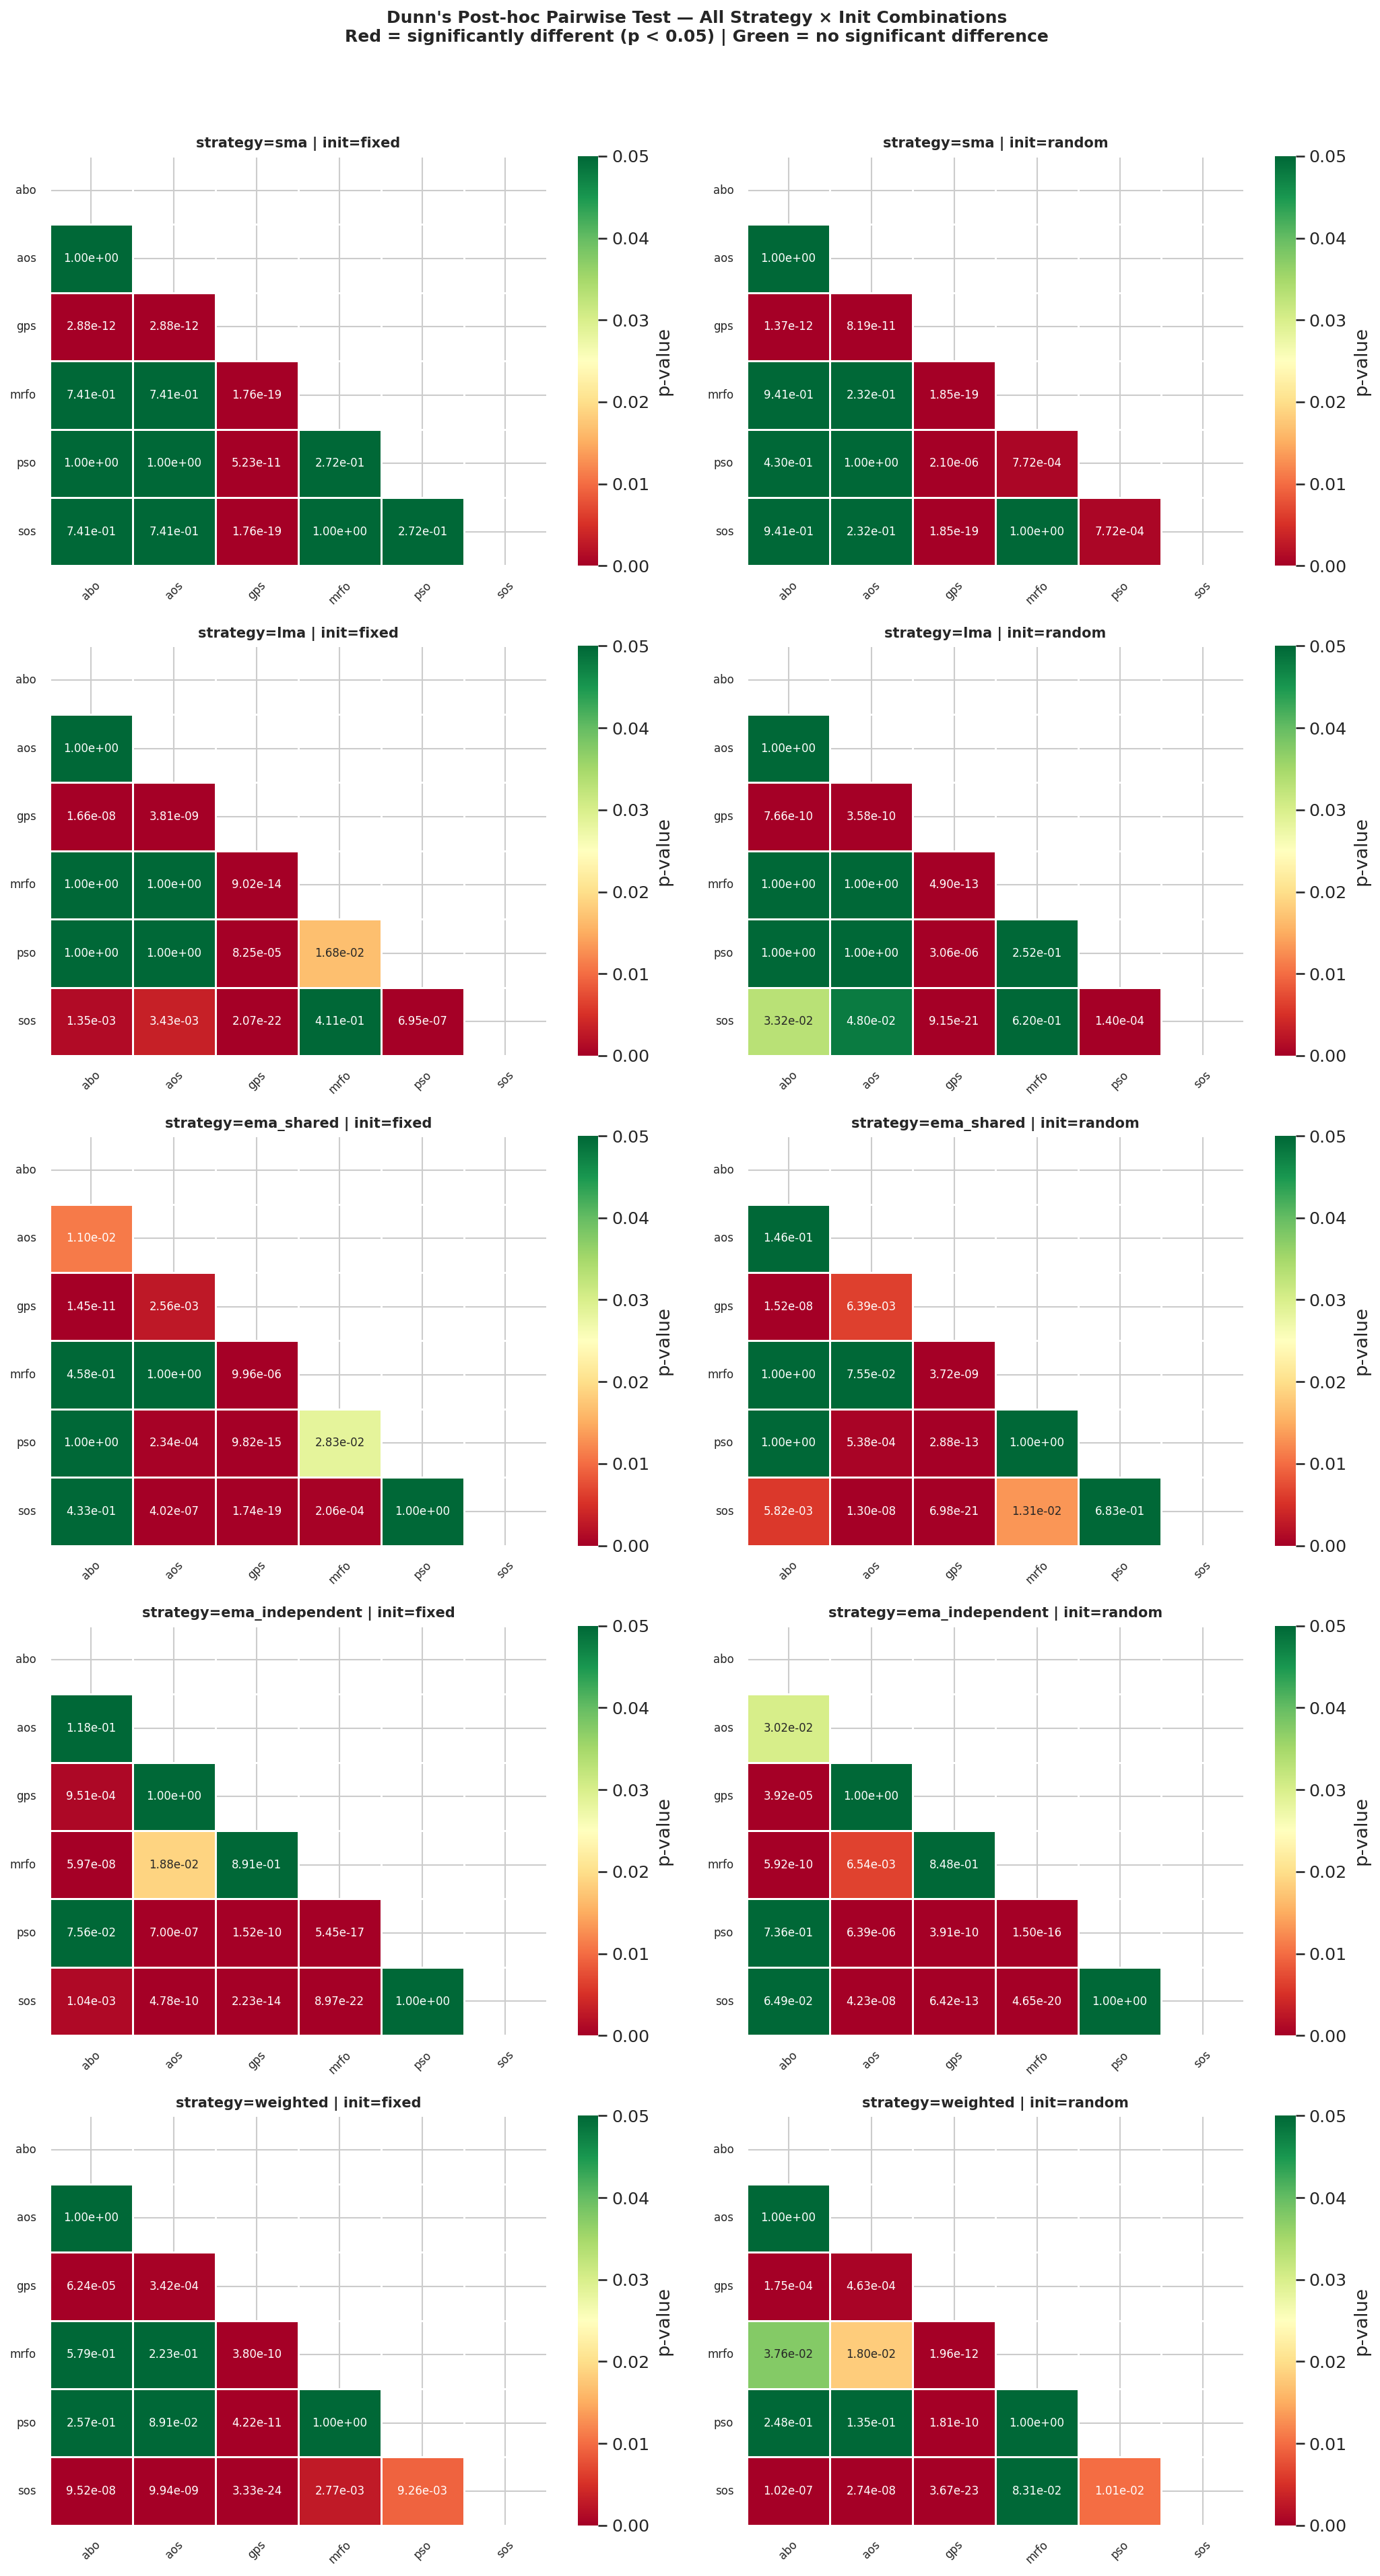
\includegraphics[width=0.5\textwidth]{images/dunn_pairwise_train.png}
  \caption{\label{fig:dunn_train}%
    Dunn's post-hoc pairwise $p$-values (Bonferroni-corrected) for all strategy
    $\times$ initialisation combinations --- training fitness. Red indicates
  significant difference ($p < 0.05$); green indicates no significant difference.}
\end{figure}
%TC:endignore

\begin{table}[h]
\centering
\caption{\label{tab:kruskal_wallis}%
Kruskal--Wallis $H$-test results comparing performance across optimization
algorithms for each strategy and initialization mode combination. All ten
configurations show statistically significant differences ($p < 0.001$),
indicating that algorithm choice meaningfully affects outcomes regardless
of strategy or initialization mode.}
\begin{tabular}{llcr}
\toprule
\textbf{Strategy} & \textbf{Start mode} & \textbf{$H$-statistic} & \textbf{$p$-value} \\
\midrule
sma              & fixed  & 119.07 & $4.95 \times 10^{-24}$ \\
sma              & random & 121.15 & $1.79 \times 10^{-24}$ \\
lma              & fixed  & 114.62 & $4.31 \times 10^{-23}$ \\
lma              & random & 106.19 & $2.62 \times 10^{-21}$ \\
ema\_shared      & fixed  & 114.93 & $3.72 \times 10^{-23}$ \\
ema\_shared      & random & 114.24 & $5.21 \times 10^{-23}$ \\
ema\_independent & fixed  & 151.73 & $5.71 \times 10^{-31}$ \\
ema\_independent & random & 144.01 & $2.51 \times 10^{-29}$ \\
weighted         & fixed  & 120.69 & $2.24 \times 10^{-24}$ \\
weighted         & random & 120.88 & $2.05 \times 10^{-24}$ \\
\bottomrule
\end{tabular}
\end{table}

The Kruskal-Wallis test was significant across all ten strategy $\times$
initialisation combinations ($p < 10^{-20}$ in every case) as per figure \ref{tab:kruskal_wallis}.
Algorithm choice has a universally
significant effect on training fitness. The \texttt{ema\_independent}
strategy ($d=4$) consistently yielded the highest $H$-statistics, suggesting
that decoupling the two EMA smoothing parameters amplifies inter-algorithm
performance differences more than further increasing dimensionality
(\texttt{weighted} at $d=14$ produced lower $H$-statistics) --- algorithms
with stronger exploration mechanisms appear to extract more from the
qualitative change in expressiveness than from raw degrees of freedom.

Four patterns emerge from Dunn's pairwise post-hoc comparisons, illustrated
in Figure~\ref{fig:dunn_train}. First, GPS is significantly worse than every
other algorithm in $8/10$ training conditions; the exceptions are on
\texttt{ema\_independent}, where MRFO collapses to the no-trade fixed point
($\$1000$, the starting balance) in $\sim 20\%$ of runs and matches GPS's
lower bound. This confirms that single-state local search struggles to
navigate the multimodal MA fitness landscape: without population diversity,
GPS converges to the nearest local optimum from its starting position. Second,
PSO, SOS, and AOS produced training-fitness distributions that were not
statistically distinguishable under Bonferroni-corrected Dunn's post-hoc
comparisons in the majority of strategy $\times$ initialisation conditions
(non-significance under Bonferroni is not formal equivalence; we report what
the test shows). Despite AOS lacking per-particle personal memory, its
shell-based exploration achieves comparable training fitness to PSO,
suggesting personal-best tracking contributes little marginal benefit
when global-best guidance is combined with structured shell diversity. Third, 
SOS exhibited unusually low within-cell variance on several conditions. Most
notably standard deviation of = \$17 across 30 random-init runs on \texttt{weighted} and
identical fitness on all 30 \texttt{sma} and \texttt{lma} runs, consistent with its
three-phase update collapsing population diversity within a small number of
iterations. SOS also requires three fitness evaluations per organism per
iteration, so if compute is taken into account for comparison it would likely
disadvantage SOS relative to PSO. Fourth, MRFO and ABO occupy intermediate
positions that vary by strategy, with no consistent dominance pattern
relative to the PSO-AOS-SOS cluster.

\subsection{Test Results --- Performance Against the Passive Baseline}

%TC:ignore
\begin{figure}[h]
  \centering
  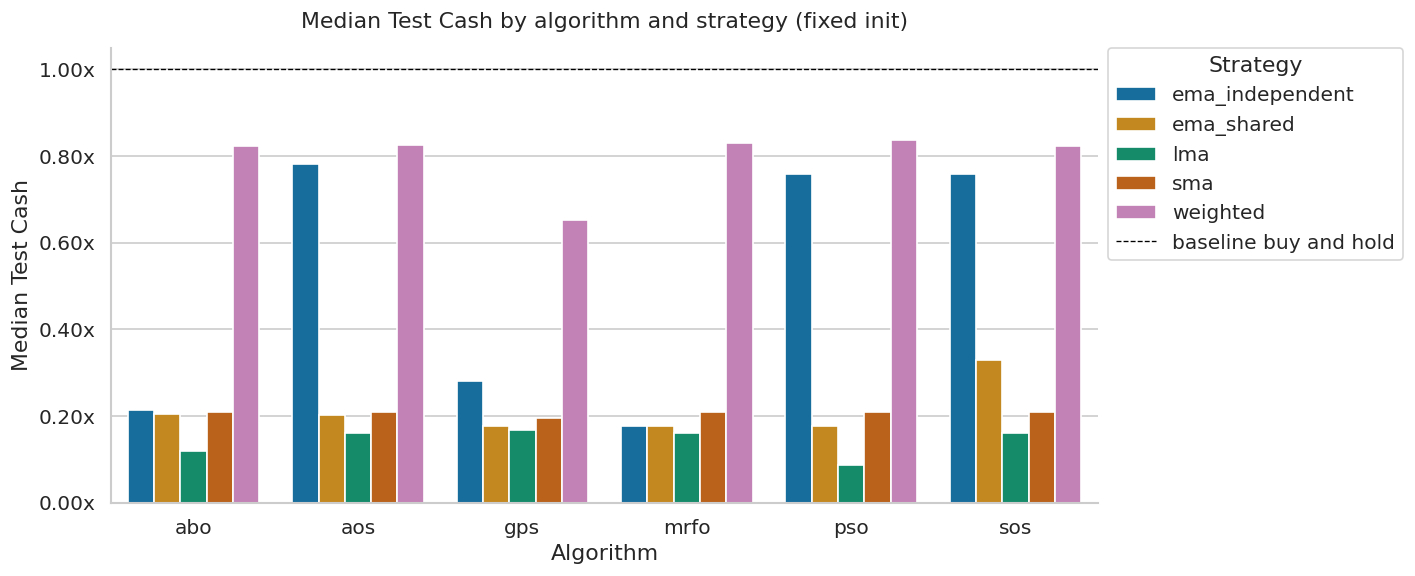
\includegraphics[width=0.95\textwidth]{images/median_test_cash_fixed.png}
  \\
  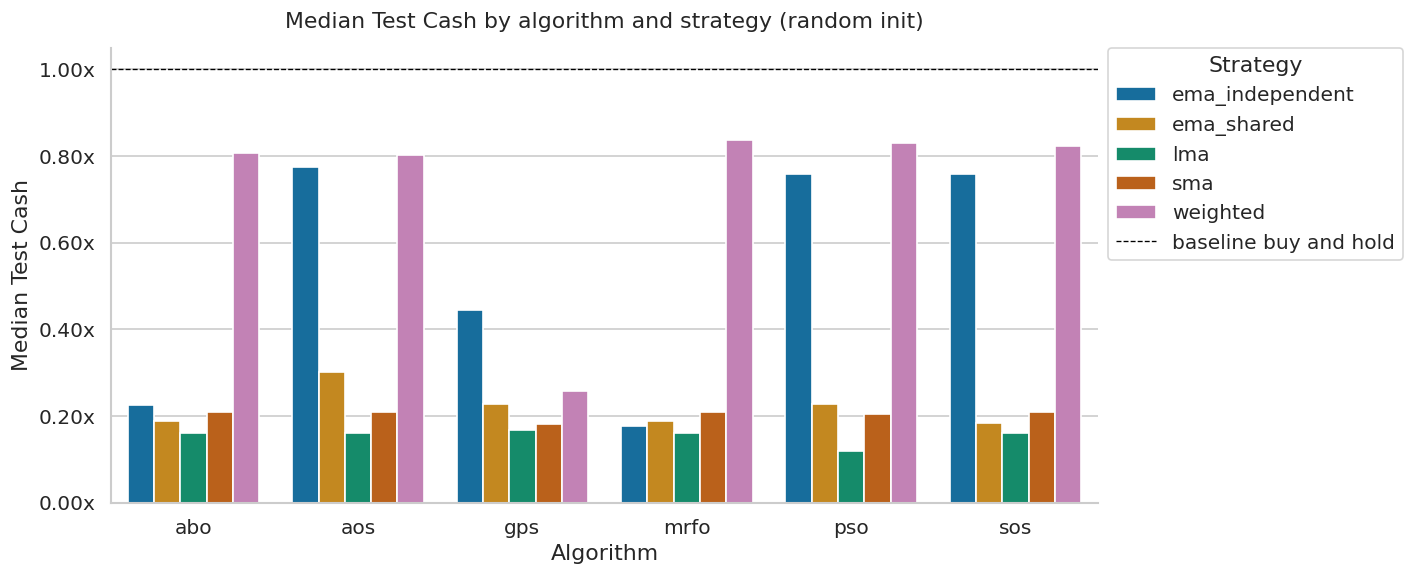
\includegraphics[width=0.95\textwidth]{images/median_test_cash_random.png}
  \caption{\label{fig:bh_median}%
    Median test cash by algorithm and strategy, normalised to the
    buy-and-hold baseline ($\$5{,}660$ from $\$1{,}000$ initial under matched
    $3\%$ entry and exit fees), for fixed (top) and random (bottom)
    initialisation. No algorithm $\times$ strategy median exceeds the
    baseline ($1.00\times$ line) under any condition.}
\end{figure}

\begin{figure}[h]
  \centering
  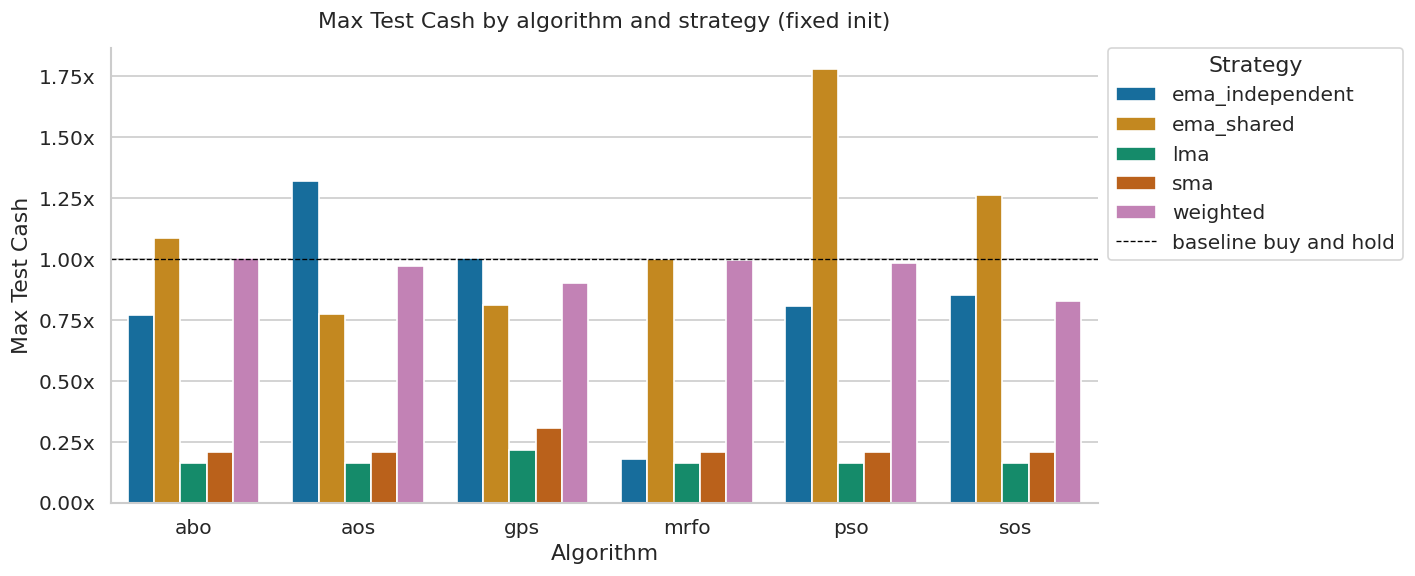
\includegraphics[width=0.95\textwidth]{images/max_test_cash_fixed.png}
  \\
  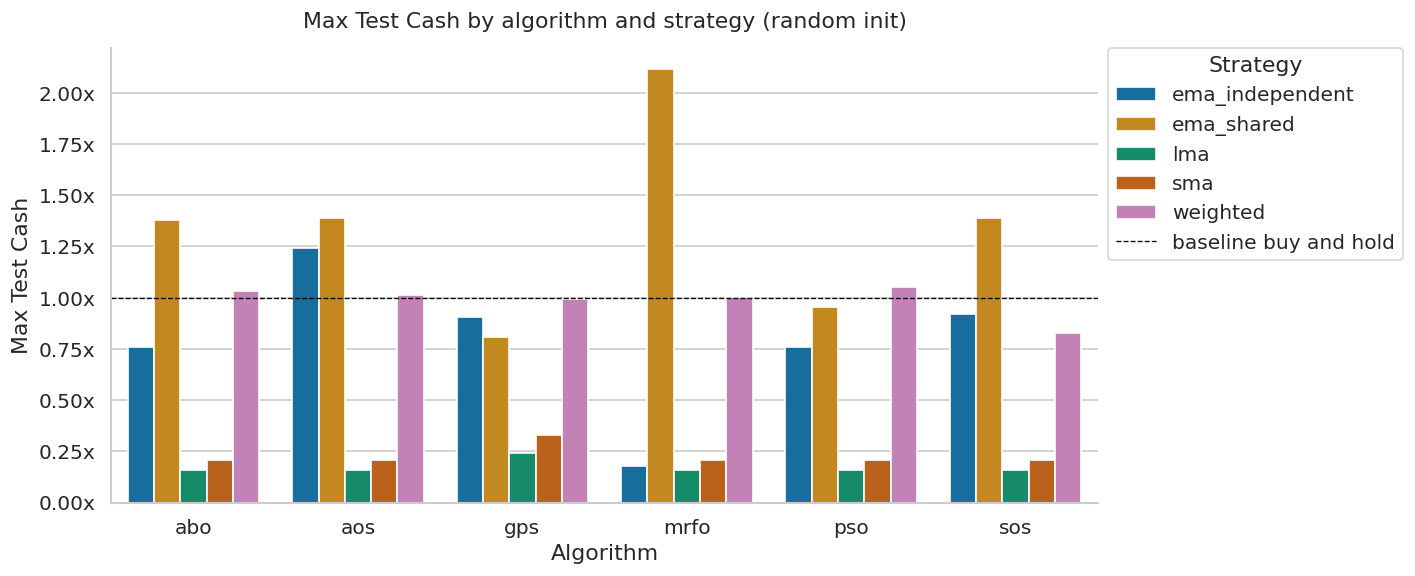
\includegraphics[width=0.95\textwidth]{images/max_test_cash_random.png}
  \caption{\label{fig:bh_max}%
    Maximum test cash by algorithm and strategy, normalised to the
    buy-and-hold baseline, for fixed (top) and random (bottom)
    initialisation. Bars above $1.00\times$ indicate at least one run in 30
    exceeded passive holding; concentration of such bars in
    \texttt{ema\_shared} reflects its long-tailed jackpot distribution
    rather than reliable optimisation.}
\end{figure}
%TC:endignore

\begin{table}[h]
\centering
\caption{\label{tab:beats_bh}%
Runs exceeding the buy-and-hold baseline ($\$5{,}660$) under strict $>$
comparison. Counts out of 30 runs per cell; 1{,}800 trials total.
One MRFO run on \texttt{ema\_shared} (fixed init) converged to exactly
$\$5{,}660.26$, matching buy-and-hold to six decimal places; it is excluded
from the strict-inequality counts but discussed below.}
\begin{tabular}{lrrrrrrrrrr}
\toprule
& \multicolumn{2}{c}{\textbf{ema\_ind}} & \multicolumn{2}{c}{\textbf{ema\_shared}} & \multicolumn{2}{c}{\textbf{lma}} & \multicolumn{2}{c}{\textbf{sma}} & \multicolumn{2}{c}{\textbf{weighted}} \\
\cmidrule(lr){2-3}\cmidrule(lr){4-5}\cmidrule(lr){6-7}\cmidrule(lr){8-9}\cmidrule(lr){10-11}
algo & fix & rnd & fix & rnd & fix & rnd & fix & rnd & fix & rnd \\
\midrule
abo  & 0 & 0 & 1 & 2 & 0 & 0 & 0 & 0 & 1 & 3 \\
aos  & 3 & 1 & 0 & 2 & 0 & 0 & 0 & 0 & 0 & 1 \\
gps  & 1 & 0 & 0 & 0 & 0 & 0 & 0 & 0 & 0 & 0 \\
mrfo & 0 & 0 & 0 & 1 & 0 & 0 & 0 & 0 & 0 & 2 \\
pso  & 0 & 0 & 2 & 0 & 0 & 0 & 0 & 0 & 0 & 1 \\
sos  & 0 & 0 & 2 & 2 & 0 & 0 & 0 & 0 & 0 & 0 \\
\midrule
\textbf{total} & \textbf{4} & \textbf{1} & \textbf{5} & \textbf{7} & \textbf{0} & \textbf{0} & \textbf{0} & \textbf{0} & \textbf{1} & \textbf{7} \\
\bottomrule
\end{tabular}
\end{table}

A passive buy-and-hold strategy over the 2020--2022 test period, with
$3\%$ broker fees, produced $\$5{,}660$ from a $\$1{,}000$ starting
balance. Of the 1{,}800 optimised bots, only 25 ($1.38\%$) strictly exceeded
this baseline; no algorithm $\times$ strategy median exceeded it under any
condition (Figure~\ref{fig:bh_median}). Win rates were heavily stratified by
strategy (Table~\ref{tab:beats_bh}): \texttt{sma} and \texttt{lma} (both
$d=2$) yielded zero wins across 720 combined runs; \texttt{ema\_independent}
($d=4$) produced $5/360$ ($1.38\%$); \texttt{weighted} ($d=14$) produced
$8/360$ ($2.22\%$); \texttt{ema\_shared} ($d=3$) produced $12/360$ ($3.33\%$).

\begin{table}[ht]
\centering
\caption{\label{tab:algo_performance_fixed}%
Statistical summary of performance metrics across combinations of algorithms 
and strategy configurations under the \texttt{fixed} start mode. 
Values represent metrics across 30 runs per cell.}
\small
\begin{tabular}{llrrrrrrr}
\toprule
\textbf{Algo} & \textbf{Strategy} & \textbf{Count} & \textbf{Mean} & \textbf{Std} & \textbf{Var} & \textbf{Min} & \textbf{Median} & \textbf{Max} \\
\midrule
abo  & ema\_independent & 30 & $1{,}482.45$ &   $994.69$ &   $989{,}410.42$ &   $858.15$ & $1{,}202.42$ & $4{,}360.90$ \\
     & ema\_shared      & 30 & $1{,}815.81$ & $1{,}391.74$ & $1{,}936{,}939.29$ &   $633.33$ & $1{,}157.60$ & $6{,}138.88$ \\
     & lma             & 30 &   $683.14$ &   $187.41$ &    $35{,}120.68$ &   $487.74$ &   $671.51$ &   $907.98$ \\
     & sma             & 30 & $1{,}172.25$ &    $12.48$ &       $155.63$ & $1{,}153.51$ & $1{,}180.28$ & $1{,}180.28$ \\
     & weighted        & 30 & $4{,}451.70$ &   $817.09$ &   $667{,}640.83$ & $1{,}130.40$ & $4{,}651.61$ & $5{,}691.01$ \\
\midrule
aos  & ema\_independent & 30 & $4{,}271.85$ & $1{,}401.70$ & $1{,}964{,}770.50$ &   $977.93$ & $4{,}425.39$ & $7{,}478.46$ \\
     & ema\_shared      & 30 & $1{,}894.03$ & $1{,}269.02$ & $1{,}610{,}421.47$ &   $603.28$ & $1{,}137.12$ & $4{,}377.15$ \\
     & lma             & 30 &   $794.10$ &   $176.29$ &    $31{,}077.99$ &   $485.41$ &   $907.98$ &   $921.28$ \\
     & sma             & 30 & $1{,}172.25$ &    $12.48$ &       $155.63$ & $1{,}153.51$ & $1{,}180.28$ & $1{,}180.28$ \\
     & weighted        & 30 & $4{,}465.42$ &   $830.24$ &   $689{,}298.14$ & $1{,}000.00$ & $4{,}676.32$ & $5{,}500.04$ \\
\midrule
gps  & ema\_independent & 30 & $2{,}328.67$ & $1{,}619.27$ & $2{,}262{,}043.67$ &   $509.80$ & $1{,}588.76$ & $5{,}684.32$ \\
     & ema\_shared      & 30 & $1{,}831.89$ & $1{,}465.63$ & $2{,}148{,}063.73$ &   $462.49$ & $1{,}000.00$ & $4{,}584.60$ \\
     & lma             & 30 &   $879.14$ &   $221.14$ &    $48{,}901.80$ &   $378.97$ &   $942.98$ & $1{,}228.54$ \\
     & sma             & 30 & $1{,}154.99$ &   $216.37$ &    $46{,}814.35$ &   $725.76$ & $1{,}104.15$ & $1{,}740.13$ \\
     & weighted        & 30 & $2{,}904.46$ & $1{,}852.43$ & $3{,}431{,}485.27$ &   $370.96$ & $3{,}688.60$ & $5{,}093.26$ \\
\midrule
mrfo & ema\_independent & 30 & $1{,}000.00$ &     $0.00$ &           $0.00$ & $1{,}000.00$ & $1{,}000.00$ & $1{,}000.00$ \\
     & ema\_shared      & 30 & $1{,}606.10$ & $1{,}366.90$ & $1{,}868{,}412.38$ &   $484.18$ & $1{,}000.00$ & $5{,}660.26$ \\
     & lma             & 30 &   $749.93$ &   $200.35$ &    $40{,}140.58$ &   $487.74$ &   $907.98$ &   $907.98$ \\
     & sma             & 30 & $1{,}180.28$ &     $0.00$ &           $0.00$ & $1{,}180.28$ & $1{,}180.28$ & $1{,}180.28$ \\
     & weighted        & 30 & $4{,}329.08$ & $1{,}145.65$ & $1{,}312{,}524.63$ & $1{,}381.96$ & $4{,}694.22$ & $5{,}644.11$ \\
\midrule
pso  & ema\_independent & 30 & $3{,}219.79$ & $1{,}460.65$ & $2{,}133{,}495.71$ & $1{,}201.23$ & $4{,}296.97$ & $4{,}565.80$ \\
     & ema\_shared      & 30 & $2{,}468.14$ & $2{,}176.03$ & $4{,}735{,}114.23$ &   $824.62$ & $1{,}000.00$ & $10{,}074.64$ \\
     & lma             & 30 &   $587.25$ &   $135.88$ &    $18{,}463.77$ &   $487.74$ &   $487.74$ &   $907.98$ \\
     & sma             & 30 & $1{,}129.06$ &   $142.71$ &    $20{,}365.10$ &   $617.37$ & $1{,}180.28$ & $1{,}180.28$ \\
     & weighted        & 30 & $4{,}813.35$ &   $460.04$ &   $211{,}639.97$ & $3{,}637.12$ & $4{,}729.43$ & $5{,}564.79$ \\
\midrule
sos  & ema\_independent & 30 & $3{,}805.27$ & $1{,}285.29$ & $1{,}651{,}977.33$ & $1{,}206.81$ & $4{,}296.97$ & $4{,}834.21$ \\
     & ema\_shared      & 30 & $2{,}237.57$ & $1{,}698.33$ & $2{,}884{,}337.13$ &   $617.00$ & $1{,}862.03$ & $7{,}142.09$ \\
     & lma             & 30 &   $907.98$ &     $0.00$ &           $0.00$ &   $907.98$ &   $907.98$ &   $907.98$ \\
     & sma             & 30 & $1{,}180.28$ &     $0.00$ &           $0.00$ & $1{,}180.28$ & $1{,}180.28$ & $1{,}180.28$ \\
     & weighted        & 30 & $4{,}580.57$ &   $477.97$ &   $228{,}457.58$ & $2{,}050.89$ & $4{,}660.90$ & $4{,}694.26$ \\
\bottomrule
\end{tabular}
\end{table}

Using fixed run as reference, according to table \ref{tab:algo_performance_fixed}., 
variance within winning strategies differed substantially.
\texttt{weighted}-strategy bots converged with median around $\$4{,}600$
to $\$4{,}730$ (for example PSO $\sigma = \$460$ | , $\mu = \$4{,}813$). In contrast,
\texttt{ema\_shared} winners came from highly dispersed distributions
(PSO $\sigma = \$2{,}176$ | $\mu = \$2{,}468$ ), consistent with random discovery rather than 
reliable optimisation: a single PSO run on this strategy
might produce $\$292$ (losing money) or \text{maximum} single instance of $\$10{,}074$, 
with little predictability from training fitness.

Referring to table \ref{tab:algo_run_details} 
two MRFO run on \texttt{ema\_shared} (fixed initialisation, run 14 and random initialisation, run 1)
converged to a test fitness of exactly $\$5{,}660.26$ matching the
buy-and-hold baseline to six decimal places but got excluded. This is not coincidence: the
optimiser identified an MA-crossover parameter set that executes precisely
one buy at the start of the test period and one sell at the end, replicating
passive holding under the matched fee structure. 

\begin{table}[ht]
\centering
\caption{\label{tab:algo_run_details}%
Detailed performance metrics of individual optimization runs, categorized by algorithm, strategy, and initialization mode.}
\small
\begin{tabular}{llcrrrr}
\toprule
\textbf{Algo} & \textbf{Strategy} & \textbf{Run ID} & \textbf{Start Mode} & \textbf{Train Final Cash} & \textbf{Test Final Cash} \\
\midrule
mrfo & ema\_shared      & 19 & random & $94{,}671.432702$ & $11{,}973.202678$ \\
pso  & ema\_shared      & 15 & fixed  & $103{,}623.884175$ & $10{,}074.639102$ \\
sos  & ema\_shared      & 14 & random & $99{,}739.498022$ & $7{,}860.381078$ \\
aos  & ema\_shared      & 25 & random & $53{,}162.066536$ & $7{,}860.381078$ \\
abo  & ema\_shared      & 6  & random & $61{,}669.572182$ & $7{,}795.072801$ \\
aos  & ema\_independent & 3  & fixed  & $8{,}387.916226$  & $7{,}478.455514$ \\
sos  & ema\_shared      & 22 & fixed  & $104{,}921.108049$ & $7{,}142.090134$ \\
aos  & ema\_independent & 1  & random & $7{,}387.991921$  & $7{,}041.993653$ \\
sos  & ema\_shared      & 4  & fixed  & $85{,}227.061950$  & $6{,}859.085979$ \\
sos  & ema\_shared      & 3  & random & $120{,}633.526793$ & $6{,}661.169413$ \\
aos  & ema\_shared      & 11 & random & $34{,}442.798674$  & $6{,}144.024916$ \\
abo  & ema\_shared      & 6  & fixed  & $82{,}411.179264$  & $6{,}138.875681$ \\
pso  & ema\_shared      & 0  & fixed  & $79{,}852.603444$  & $6{,}128.390758$ \\
pso  & weighted        & 28 & random & $13{,}408.479220$  & $5{,}965.439091$ \\
abo  & ema\_shared      & 14 & random & $76{,}429.269569$  & $5{,}906.325814$ \\
abo  & weighted        & 9  & random & $10{,}015.651104$  & $5{,}853.488490$ \\
abo  & weighted        & 24 & random & $10{,}757.072994$  & $5{,}767.026518$ \\
aos  & ema\_independent & 28 & fixed  & $6{,}960.173097$  & $5{,}744.356481$ \\
aos  & weighted        & 6  & random & $11{,}633.609194$  & $5{,}737.972241$ \\
abo  & weighted        & 8  & fixed  & $11{,}447.583852$  & $5{,}691.006969$ \\
gps  & ema\_independent & 4  & fixed  & $7{,}365.586603$   & $5{,}684.316408$ \\
mrfo & weighted        & 20 & random & $11{,}545.351863$  & $5{,}680.524618$ \\
abo  & weighted        & 23 & random & $10{,}582.572136$  & $5{,}677.242799$ \\
aos  & ema\_independent & 7  & fixed  & $6{,}152.365887$  & $5{,}675.507260$ \\
mrfo & weighted        & 14 & random & $11{,}877.068017$  & $5{,}670.184694$ \\
mrfo & ema\_shared      & 14 & fixed  & $79{,}302.563503$  & $5{,}660.263187$ \\
mrfo & ema\_shared      & 1  & random & $49{,}408.611819$  & $5{,}660.263187$ \\
\bottomrule
\end{tabular}
\end{table}

\subsection{Test Results --- Statistical Differentiation}

%TC:ignore
\begin{figure}[h]
  \centering
  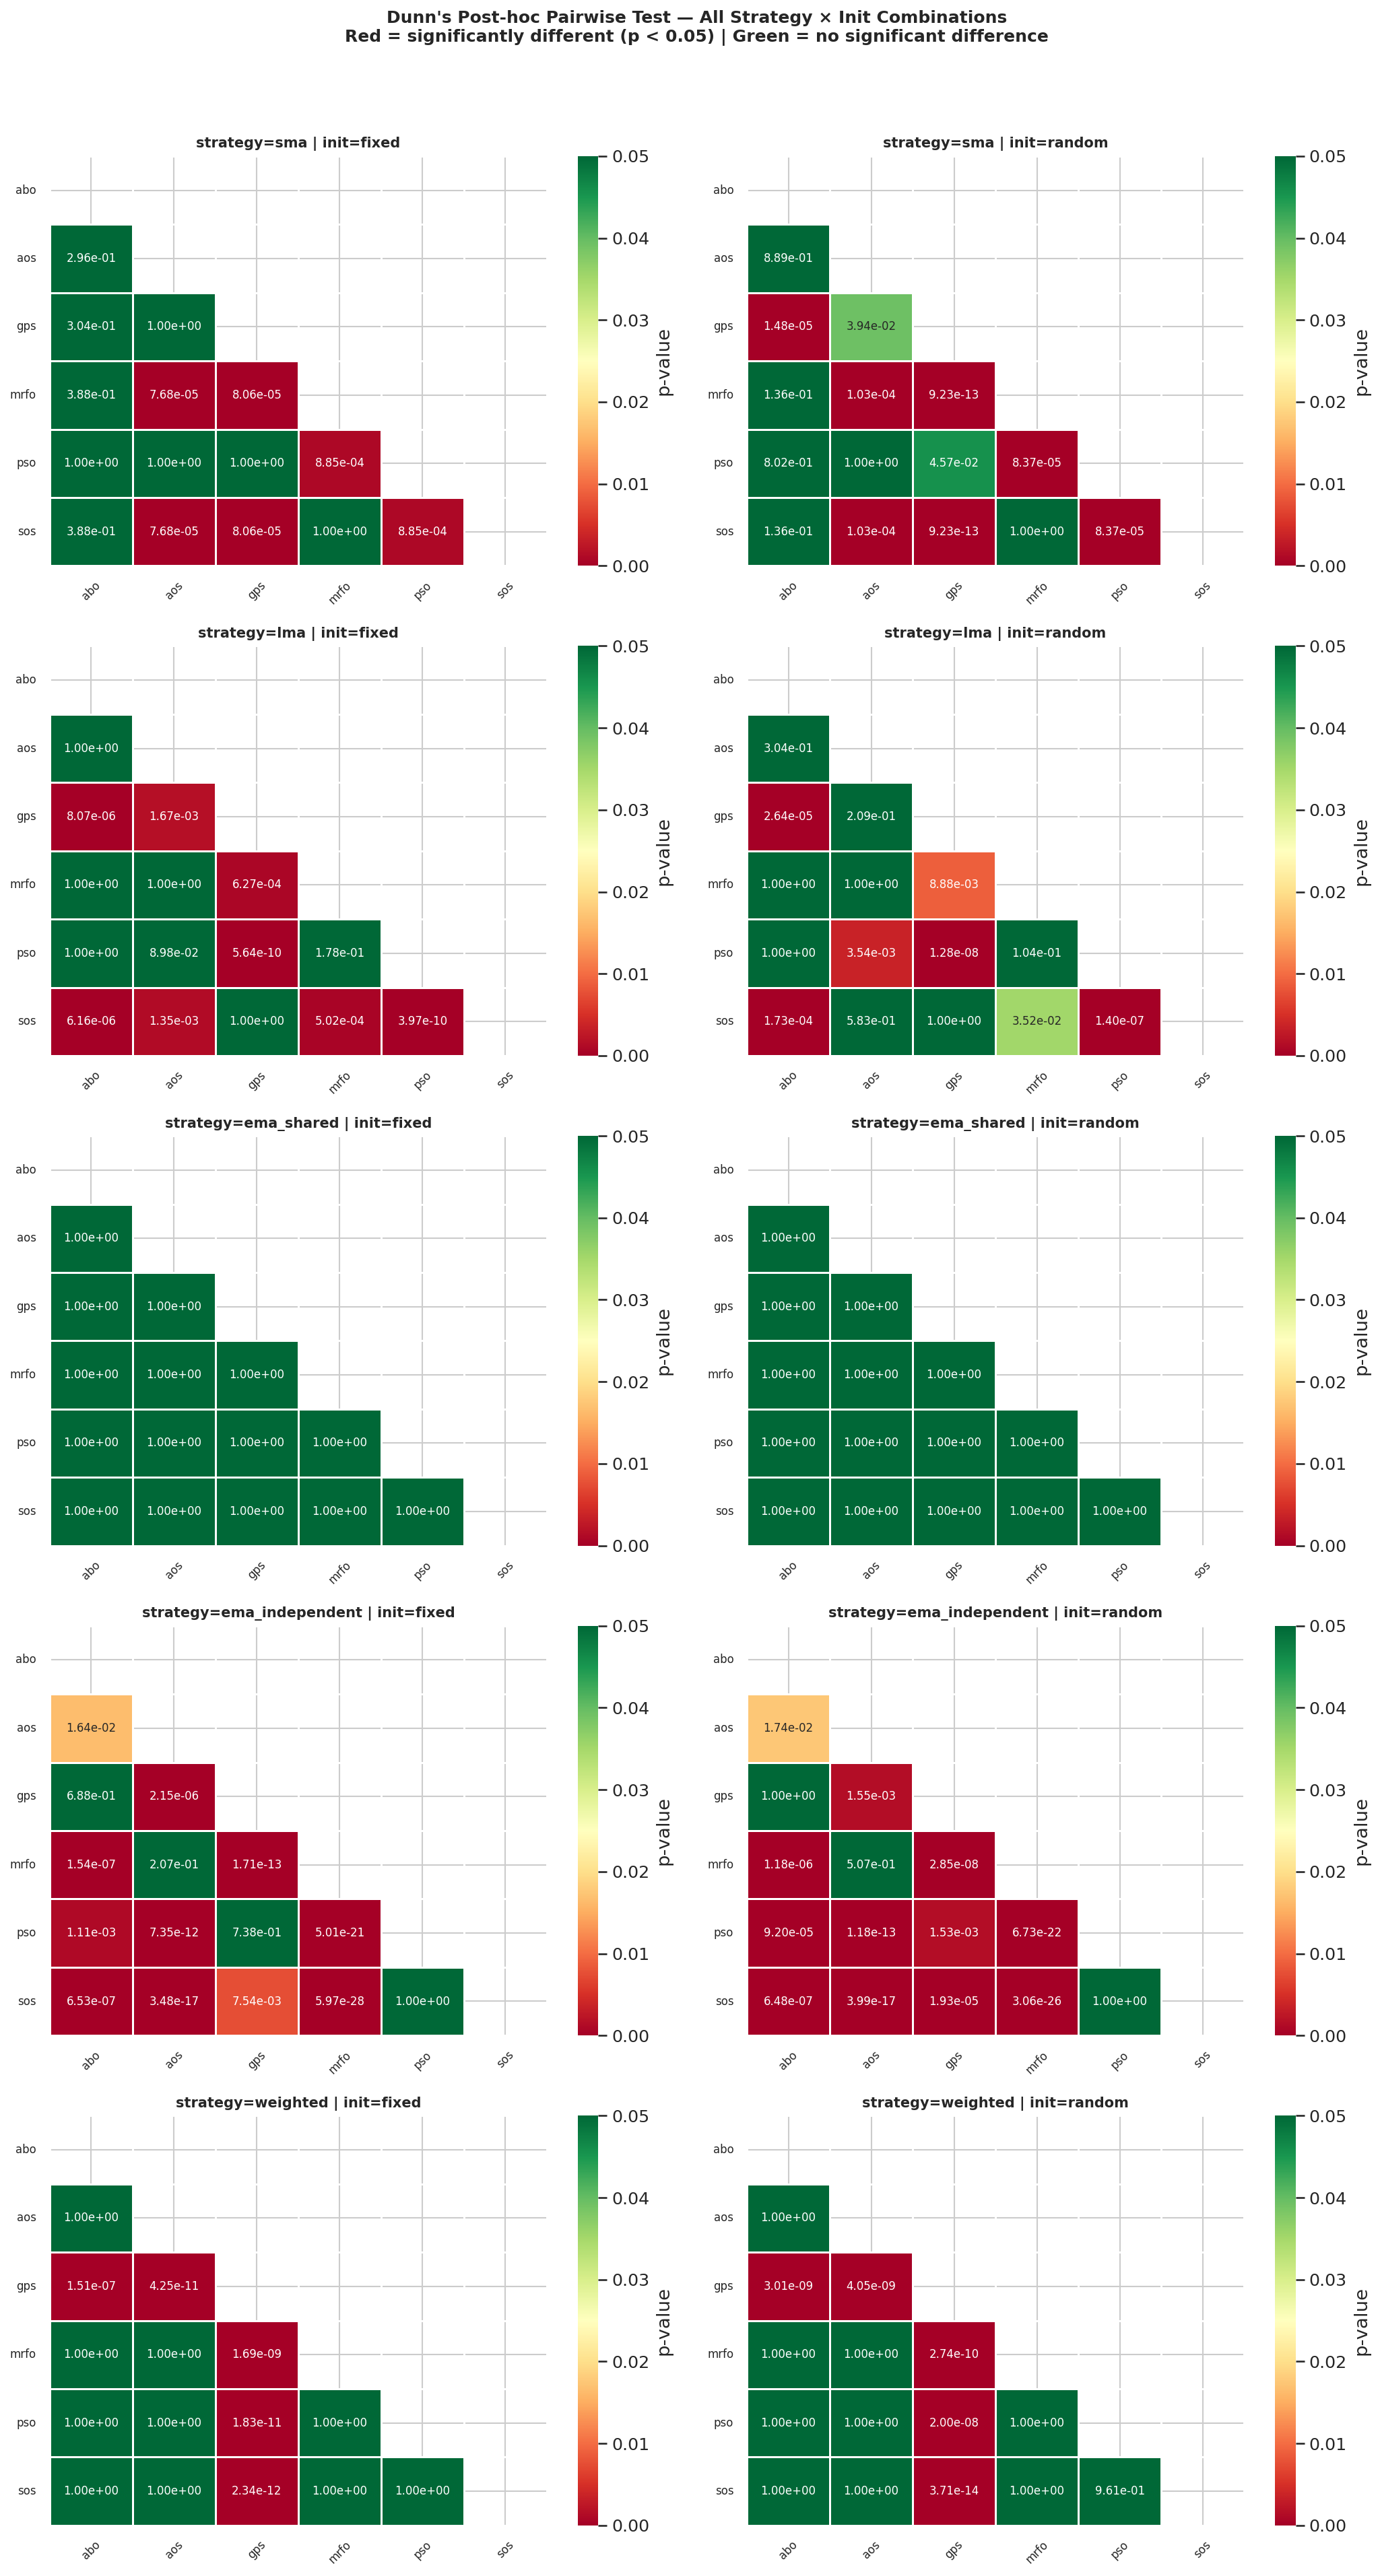
\includegraphics[width=0.5\textwidth]{images/dunn_pairwise_test.png}
  \caption{\label{fig:dunn_test}%
    Dunn's post-hoc pairwise $p$-values (Bonferroni-corrected) for all strategy
    $\times$ initialisation combinations --- test fitness.}
\end{figure}
%TC:endignore

On test data, the significant pairwise differences observed during training
largely disappear (Figure~\ref{fig:dunn_test}). The most extreme case is
\texttt{ema\_shared}: under both fixed and random initialisation, every
pairwise $p$-value equals $1.000$. All six algorithms produce statistically
indistinguishable test fitness distributions. The algorithms that were most
differentiated during training, particularly the PSO-SOS-AOS cluster
versus GPS converge to similar test performance across strategies.
The exception is \texttt{lma} fixed initialisation, where GPS achieves the
highest test median ($\$948$) of all six algorithms. Inspecting GPS,
the test median ($\$948$ lma and $\$1056$ sma) is actually higher
than train median ($\$445$ lma and $\$572$ sma) this might indicate
either (i) coincidence from fixed point initialization or (ii) the greedy
local search nature incidentally helped GPS to have better generalization.

\subsection{Why Training Fitness Did Not Predict Test Fitness}

%TC:ignore
\begin{figure}[h]
  \centering
  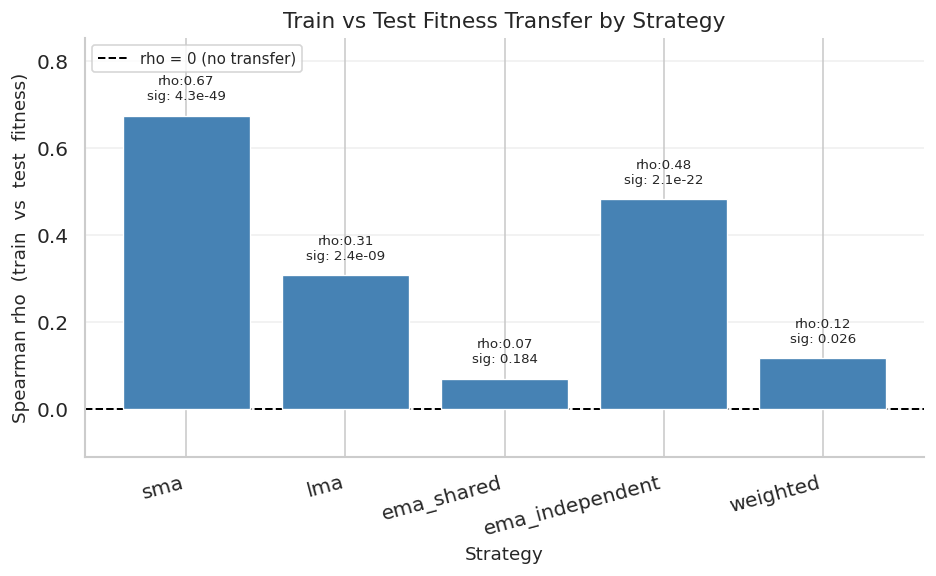
\includegraphics[width=0.7\textwidth]{images/train_test_spearman.png}
  \caption{\label{fig:spearman}%
    Spearman rank correlation between training and test fitness per strategy
    (both initialisation modes pooled, $n=360$ per strategy).
    $\rho = 0$ corresponds to no rank transfer.}
\end{figure}
%TC:endignore

Train--test rank correlation (Spearman's $\rho$ on per-run fitness pairs,
both initialisation modes combined) reveals a structural pattern
(Figure~\ref{fig:spearman}). \texttt{sma} ($d=2$) shows $\rho = 0.67$: 
if an optimiser ranks high on training, it ranks high on
test. \texttt{ema\_independent} ($d=4$) shows $\rho = 0.48$,
indicating moderate but reliable transfer. \texttt{lma} ($d=2$) follows at
$\rho = 0.31$. \texttt{weighted} ($d=14$) is weak and only marginally
significant ($\rho = 0.12$, $p = 0.026$). \texttt{ema\_shared} ($d=3$) shows
no detectable transfer ($\rho = 0.07$, $p = 0.18$, n.s.).

The relationship is not strictly monotonic in dimensionality:
\texttt{ema\_shared} ($d=3$) has worse transfer than \texttt{weighted}
($d=14$), and the difference between \texttt{ema\_shared} and
\texttt{ema\_independent} is a single additional parameter, decoupling the
two EMAs' smoothing rates but produces a sevenfold change in $\rho$.
This indicates that the \emph{nature} of the parameterisation matters as
much as its size: a tightly-coupled $d=3$ space can produce less generalisable
optima than a decoupled $d=4$ space or even a $d=14$ weighted combination.

Ironically, the two strategies with the most test-set wins (\texttt{ema\_shared}: 13;
\texttt{weighted}: 8) are also the two with the lowest train--test
correlations. Their wins represent stochastic discovery, not reliable
optimisation: a reading of $\rho = 0.07$ should not expect any
optimiser's training performance to inform its test outcome on
\texttt{ema\_shared}. The strategies where training rank \emph{does} predict
test rank (\texttt{sma}, \texttt{ema\_independent}, \texttt{lma}) are
predictably mediocre on test meaning their best-training algorithm is also their
best-test algorithm, but neither beats the baseline. This is the
descriptiveness-versus-search-space trade-off realised empirically: higher
expressiveness produced higher training fitness ($\$100{,}000{+}$ medians on
\texttt{ema\_shared}) but transferred no useful information to held-out test data.

\subsection{Interpretation}

Two non-exclusive explanations account for the failure of training fitness to
generalise. The first is overfitting to the training market regime:
parameters optimised on the pre-2020 BTC market exploit structural patterns
--- momentum cycles, volatility regimes --- specific to that period. The
COVID-19 crash, the 2021 bull run, and the 2022 bear market introduce
qualitatively different dynamics that these parameters are not positioned to
exploit.

The second explanation is that MA crossover signals are fundamentally weak
predictors of BTC price movement across diverse regimes regardless of how
precisely the parameters are tuned; if strategy expressiveness is the
binding constraint, no optimiser can recover transferable advantage from the
parameter space. The $1.44\%$ rate of bots exceeding buy-and-hold across
1{,}800 trials is statistically consistent with random sampling from the
strategy-fitness right tail, and does not provide evidence of a learnable
trading edge under the MA-crossover hypothesis space. This is consistent
with --- though does not formally test --- the efficient market hypothesis
for short-horizon technical signals on highly liquid assets.